%!Mode:: "TeX:UTF-8"
% \documentclass[12pt]{article}
\documentclass[aps,prd,superscriptaddress,nofootinbib,preprint]{ctexart}
%\usepackage{CJK}
\usepackage[]{graphicx}
\usepackage{subfigure}
\usepackage[T1]{fontenc}
\usepackage{amsmath}
\usepackage{color}
\usepackage{indentfirst}
\usepackage{fancyhdr}
\usepackage{lastpage}
\usepackage{float}
\usepackage{enumerate}
%\usepackage{nopageno}
\newcommand{\wuhao}{\fontsize{10pt}{10pt}\selectfont}
%\usepackage[fntef]{ctexcap}
%\CTEXsetup[number={\chinese{section}},format={\Large\bfseries}]{section}
\begin{document}
\setlength{\parindent}{2em}
%\pagestyle{fancy}
%\fancyhf{}
%\rfoot{\thepage\ of \pageref{LastPage}}
\renewcommand{\headrulewidth}{0pt}

\begin{CJK}{UTF8}{gbsn}

\title{宇生缪子探测器蒙特卡洛模拟环境的初步搭建}

\author{罗鑫}
\affiliation{中山大学物理学院,广州南校园,510275, 中国}
\author{许伊欣}
\affiliation{中山大学物理学院,广州南校园,510275, 中国}
\author{曹广杰}
\affiliation{中山大学数据与计算机学院,广州东校园,510275,中国}
\author{唐健\footnote{通讯作者:tangjian5@mail.sysu.edu.cn}}
\affiliation{中山大学物理学院,广州南校园,510275, 中国}



\begin{abstract}
 本文首先介绍宇宙射线产生高能缪子(简称宇生缪子)的物理过程,重点关注教学实验室利用偶然符合计数法探测缪子数的基本工作原理。
 其次,我们引入探测器蒙特卡洛模拟的方法,考虑了完整的物理过程模拟,优化探测器材料和几何形状,并实现探测器模拟结果的输入与输出功能。
 最后,我们讨论了探测器模拟的初步结果,初步获得了缪子寿命测量的谱形,为后续探测器的搭建奠定基础。
\end{abstract}

\maketitle

\section{研究背景介绍}
\subsection{蒙特卡罗模拟在国内外高能物理实验的重要性}

蒙特卡罗(Monte Carlo简写MC)方法,又称计算机随机模拟方法,最早用于第二次世界大战时美国洛斯阿拉莫斯实验室(LANL)的”曼哈顿计划“中设计核武器的统计计算~\cite{6}。蒙特卡洛方法具体而言是基于具体问题的概率模型等特征,模拟实验过程的步骤,通过数学模拟实验对已有的概率分布进行抽样分析,由此获得模拟数据的实验方法。伴随着计算机的性能的提高和蒙特卡罗方法研究的深入和应用范围的扩大,高能物理领域的粒子探测系统模拟越来越需要使用蒙特卡洛模拟的方法。与通过构建和求解主要粒子的辐射方程以及输运方程相比较,蒙特卡洛方法可以更加关注概率统计模型的构建,而且多次重复实验的工作比如使用随机数(或伪随机数)对随机变量抽样,大多都由计算机完成。之后再根据获得的实验结果以及模型的预测,从而明确出数据中隐藏的特性。总体上,基于统计学的思想来获得所求解的数学期望等值,以此来推测实验可能出现的结果。\\

探测器的蒙特卡洛模拟主要为了对探测器性能进行优化,确定数据获取中触发判断选择逻辑,估计实验所能达到的物理目标以及解释和预测实验结果。所以模拟程序必须精确地描述探测器的几何结构,模拟粒子与探测器介质的物理过程,以获得一定程度可以信服的模拟结果~\cite{7}。当前大多数模拟程序都是基于Geant4软件框架~\cite{Agostinelli:2002hh}。例如,欧洲大型强子对撞机实验(LHC)的各类子探测器ATLAS~\cite{Aad:2010ah}, CMS~\cite{Abdullin:2011zz}, ALICE~\cite{Hrivnacova:2011zz}和LHCB~\cite{Clemencic:2011zza}等大量使用计算机、模拟探测器响应。类似地,加速器中微子振荡实验如T2K~\cite{Abe:2011ks},NoVA~\cite{Ayres:2004js}等模拟中微子信号和本底鉴别过程。我们拟搭建小型教学设备用于宇生缪子的探测,需对探测器的结构进行优化,为此我们搭建了基于Geant4开发的探测器模拟程序。

\subsection{Geant4介绍}

Geant4是欧洲核子中心(CERN)研制开发的一个大型高能物理探测器模拟程序,是采用当代先进的面向对象程序设计技术利用C++语言编写~\cite{1}。该软件包提供了高能物理模拟实验探测器的必要工具,利用探测器几何结构的相关类,用户能够精确地定义复杂探测器的材料和几何结构,利用物理过程的相关类,通过对不同粒子注册相关的物理过程,用户能够模拟所有己知的粒子与探测器介质之间的各种可能的相互作用,同时可以用不同可视化引擎查看探测器的几何结构以及粒子在探测器中的径迹,方便初学者了解探测器模拟。同时,用户可以定义不同的“动作”(Action)类来控制模拟过程相应的层面的行为或者输出所产生的数据~\cite{7}。

\subsection{缪子探测的教学意义}

Geant4模拟程序的设计旨在为宇生缪子探测器搭建实验提供指导。宇生缪子探测器的搭建具有重大教学意义。在理论方面,宇生缪子探测实验有助于学生理解宇宙中高能缪子的产生过程,而缪子寿命的测量可以间接验证狭义相对论中的时间膨胀效应或者确定粒子物理标准模型中的费米耦合常量。在实验技术方面,缪子探测器的搭建涉及探测器设计与模拟,核电子学,探测器与电子学刻度,在线获取系统和数据离线分析等方法~\cite{2}。学生在自主组建实验装置可以对探测器的结构有新的认识,模拟实验过程可以接触面向对象的编程技术,了解到计算机模拟对实验的指导性作用。
\section{缪子探测器基本工作原理}
\subsection{缪子简介}

缪子是一种类似电子的基本粒子,属于带电轻子,$\mu^-$带有一个单位负电荷,自旋为$\frac{1}{2}$的费米子,相比电子,它的质量更大,为$105. 658$ MeV$/c^2$,是电子质量的207 倍。$\mu^-$的反粒子为$\mu^+$,带有一个单位正电荷~\cite{3}。缪子的平均寿命约为$2.2\mu s$, 准确值为2.1969811(22)$\times10^{-6}$ s,缪子的衰变方式~\cite{4}:
\begin{align}
\mu^- \rightarrow e^- + \nu_\mu + \bar\nu_e\\
\mu^+ \rightarrow e^+ + \bar\nu_\mu + \nu_e
\end{align}

由于在当前研究项目下,无法鉴别$\mu^-$和$\mu^+$,所以在下文没有特别提示,$\mu^-$和$\mu^+$统称为缪子。到达地球表面的缪子绝大部分不是来自宇宙射线,而是由宇宙射线中高能质子撞击大气层顶部,产生 $\pi^\pm$ 介子,然后 $\pi^\pm$ 介子会在传输较短的距离后衰变,产生缪子($\pi^- \rightarrow \mu^- + \bar\nu_u ,\ \pi^+\rightarrow \mu^+ + \nu_\mu$)。 如果不考虑相对论效应,这些缪子的传输距离约为468米(2.197 $\mu$s$\times \ln(2) \times 0.9997\times$c)。由于相对论性效应的存在,高速运动的缪子寿命会乘以洛伦兹因子(由缪子运动速度决定)。从而,该传输距离将被拉长,足以支持缪子到达地球表面~\cite{3}。

\subsection{塑料闪烁体}

闪烁体是一种能够吸收高能粒子或射线并发出光子的材料。其中塑料闪烁体是有机闪烁物质在塑料中的固溶体,通常由基质、闪烁物质及波长位移剂组成,塑料闪烁体中的基质(例聚苯乙烯)起着能量转移作用,可吸收能量,然后转移给闪烁分子,使闪烁效率提高。波长位移剂可以改变光的波长,使闪烁分子输出的光波长落在光电倍增管敏感区域,改善信号输出。$\mu^\pm$穿过闪烁体的时候,会能量损失,失去的能量会被闪烁体吸收,然后产生光子,光子就会被光电倍增管所探测到,形成电信号,就能在示波器上看到。

\subsection{符合法测量宇生缪子}

在粒子物理实验中,对于平均寿命大于 $10^{-9}s$的不稳定粒子, 传统的粒子寿命测量方法是直接测量衰变事例的时间分布, 计算出粒子的寿命。实验上通常采用延迟符合法测量$\mu$子的平均寿命。该方法至少需要2个探测器以及相关的逻辑电路和数据处理系统~\cite{5}。\\
宇宙射线中的μ子通过塑料闪烁体时,主要的能量损失方式是电离能损,并伴随库伦散射。高能量μ 子可直接从闪烁体中穿出,并在径迹周围产生电子及荧光光子等次级粒子;一些较低能量μ子在闪烁体中停止后,可以自由衰变,也可能与物质的原子核发生作用被俘获而消失。以$\mu^+$为例,衰变过程
$\mu^+ \to e^+ + \nu_e + \bar{\nu}_{\mu}$
,产生的电子($e^+$)继续与闪烁体发生作用损失能量并使闪烁体分子激发,而电子中微子和$\mu$型反中微子直接穿出。塑料闪烁体中受激发的分子在极短时间内退激发并发射荧光(荧光波长在300-500nm之间)荧光通过光电倍增管光电转化放大而输出电信号,这个信号将作为$\mu^+$的`` 到达''信号。当停止在闪烁体内的$\mu^+$子发生衰变, 产生的电子被闪烁探测器探测,形成$\mu^+$“衰变”的信号。“到达”探测器的信号与$\mu^+$“衰变”信号的时间间隔,即为$\mu^+$衰变的寿命。

\section{缪子探测器MC模拟}

我们设计基于Geant4的缪子探测器模拟程序,包括了初级事例的产生,探测器几何信息,入射粒子的物理过程,击中信息及其数字化,模拟事例的输出。图\ref{gen}是我们设计的程序的整体结构\\
\begin{figure}[h]
    \centering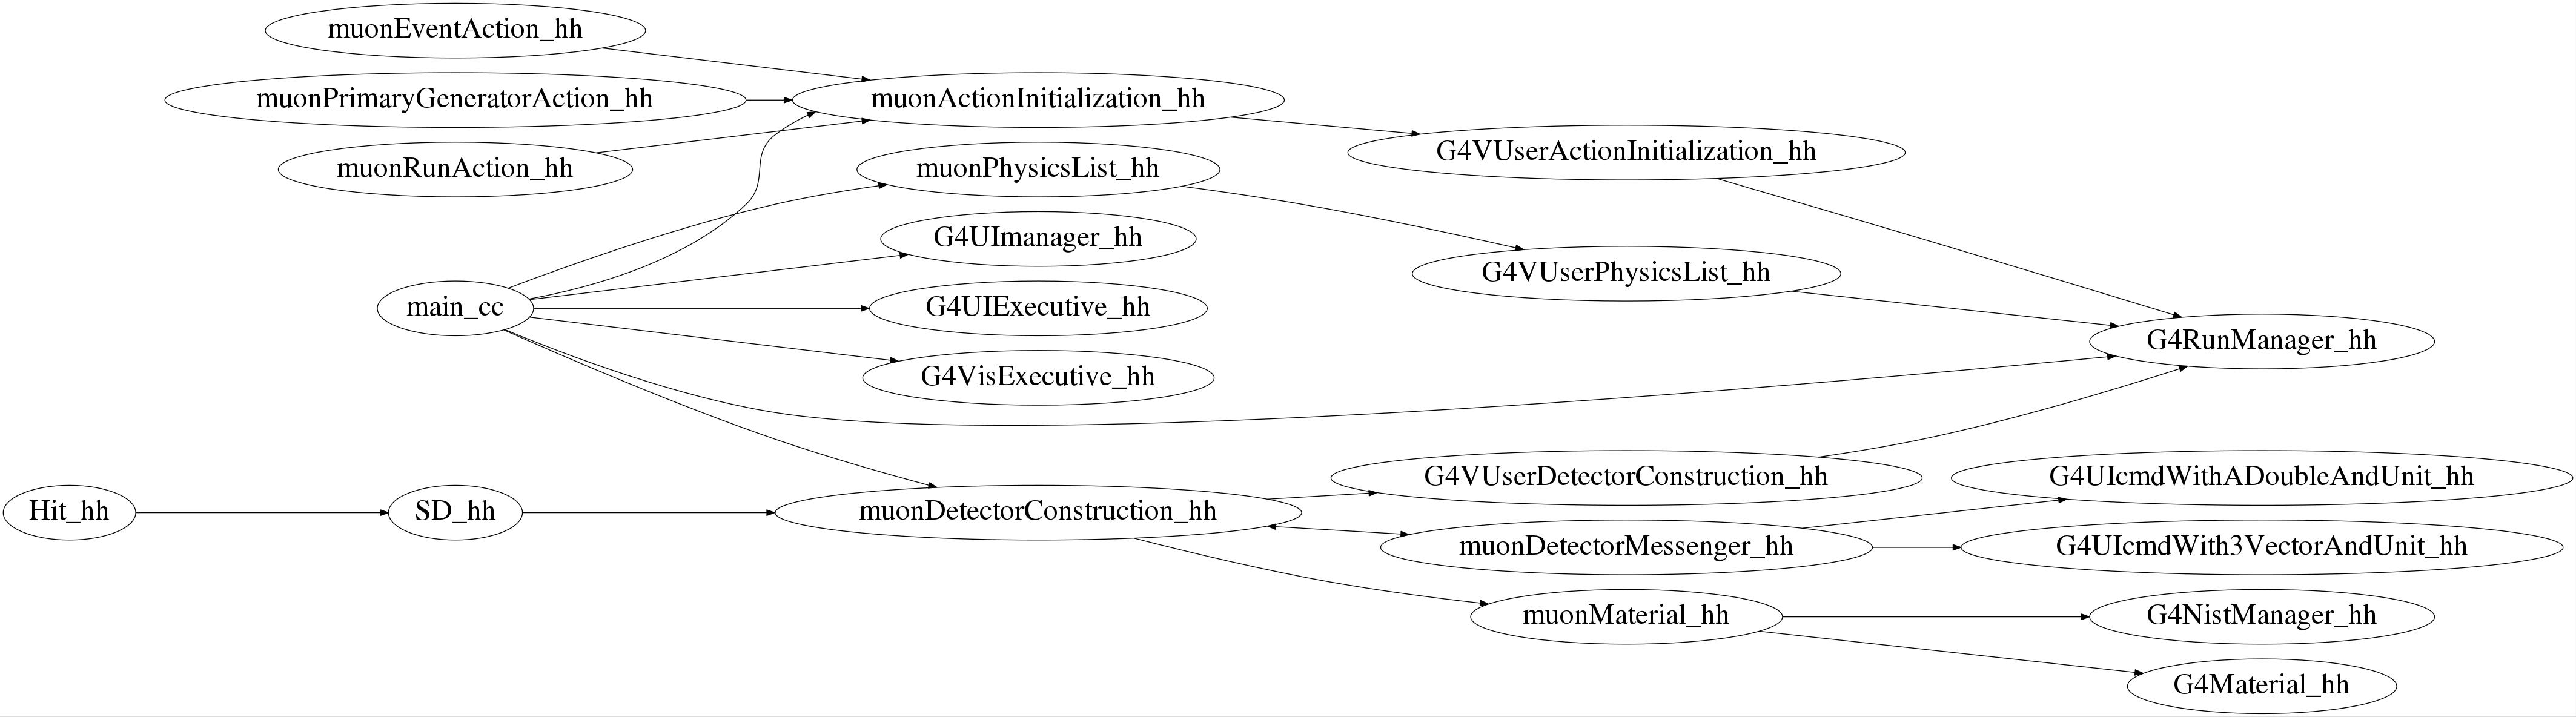
\includegraphics[width=\textwidth]{pic/main.jpg}
    \caption{程序的整体结构框图}\label{gen}
\end{figure}


主函数main.cc会新建 Geant4 的 G4RunManager 对象,由 G4RunManager 控制 G4VUserPhysicsList ,G4VUserDetectorConstruction,G4VUserActionInitialization 类,它们分别是muonPhysicsList ,muonDetectorConstruction,muonActionInitialization 三个对象的基类,而这三个对象作用分别是 muonDetectorConstruction 描述探测器几何信息, muonPhysicsList 描述粒子的物理过程,muonActionInitialization 控制获取信息的管理对象。

muonActionInitialization 控制 muonEventAction, muonPrimaryGeneratorAction, muonRunAction。 它们作用分别是用于控制初级粒子动力学信息的  muonPrimaryGeneratorAction 类,用于控制程序开始和结束操作的 muonRunAction 类和用于数据输出及击中信息数字化的 muonEventAction 类。

在探测器几何搭建相关的类中,muonMaterials是控制探测器的材料信息,muonDetectorMessenger 是用户交互控制探测器位置,尺寸信息。

\subsection{探测器材料和几何}

如图\ref{maAge}所示,探测器由两块梯形板构成。每块梯形板的高为338.5mm,下底长143.5mm,上底长84mm,厚度为20mm。探测器板的材料为蒽,分子式为C14H10,折射率设置为1.3,光子在其中的衰减长度设置为3m.在实际实验中,为保证高能粒子穿过闪烁体时产生的闪烁光尽可能地被光电倍增管收集到,会在探测器板的表面包裹反光材料,因此在模拟程序中,两块探测器板都覆盖了1mm厚的氧化铝反射层,其反射率设置为1,折射率为1.76,光子在反射层中的衰减长度为1m。(上底面没有覆盖反射层因为光电倍增管的光窗处在上底面的位置)。探测器上表面设置了应该接受面,将它对光子吸收率为1,用于记录从探测器射出的光子信息。

\begin{figure}[h]
    \centering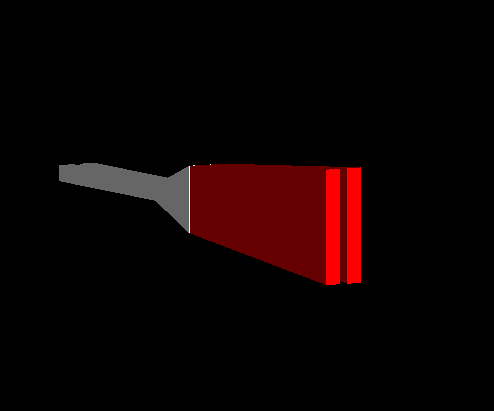
\includegraphics[width=0.8\textwidth]{pic/muonde1.png}
    \caption{探测器几何示意图}\label{maAge}
\end{figure}

\subsection{探测器模拟的输入输出和物理过程}


探测器模拟的输出为探测器的上表面会输出光子的到达时间以及光子的能量信息。探测器本身会输出缪子到达时间,缪子的位置信息和沉积的能量信息,可以通过缪子的位置信息判断缪子是否衰变。探测器模拟输入信息可以更改探测器的厚度和位置,也可以更改入射粒子的类型和能量。默认是厚度是20mm,相距10mm,入射粒子是$\mu^-$。\\

缪子从探测器上方75mm射入搭建的世界。在进入探测器之前,缪子在空气中传输并经历电离过程。在此过程中,缪子损失能量并将周围原子、分子中的电子电离。在Geant4中,此电离过程由G4MuIonisation类控制。
缪子在反射层处会损失一定能量并将损失的能量以光子的形式释放。这个过程由G4Transportation类控制。
缪子在闪烁体中使其轨迹周围分子中的电子发生电离,电离中产生的电子会与闪烁材料发生相互作用并释放光子。该过程由G4Scintillation类控制。
能量较高的缪子可直接从闪烁体中穿出,但是一些能量较低的缪子会在闪烁体中发生衰变反电子型中微子、缪子型中微子以及电子。反电子型中微子和缪子型中微子经历输运过程,此过程由Geant4中的G4Transportation类控制。电子在闪烁体中减速运动产生轫致辐射释放光子,此过程由G4eBremsstrahlung类控制。当电子在闪烁体中的运动速度大于光波在此介质中的相速时,会产生切伦科夫辐射释放光子,此过程由G4Cerenkov类控制。除了轫致辐射和切伦科夫辐射以外,缪子衰变产生的电子还会经历电离过程并且与闪烁体发生相互作用,这两个过程分别由G4eIonisation和G4Scillination类控制。附录给出一个$\mu^-$粒子为例,模拟输出单个事例历经的物理过程的列表


\section{缪子探测器模拟初步结果分析}
\subsection{探测器优化}

我们利用该程序测试了厚度都是为20mm的两个探测器的性能,将它们相距10mm,其中包括两个反射层的厚度,入始粒子的能量从10MeV到69MeV均匀分布,每个缪子能量都运行了1000个事例。然后计算缪子的穿透距离和沉积能量以及单位距离的沉积能量的平均值和方差。\\

\begin{figure}[H]
    \centering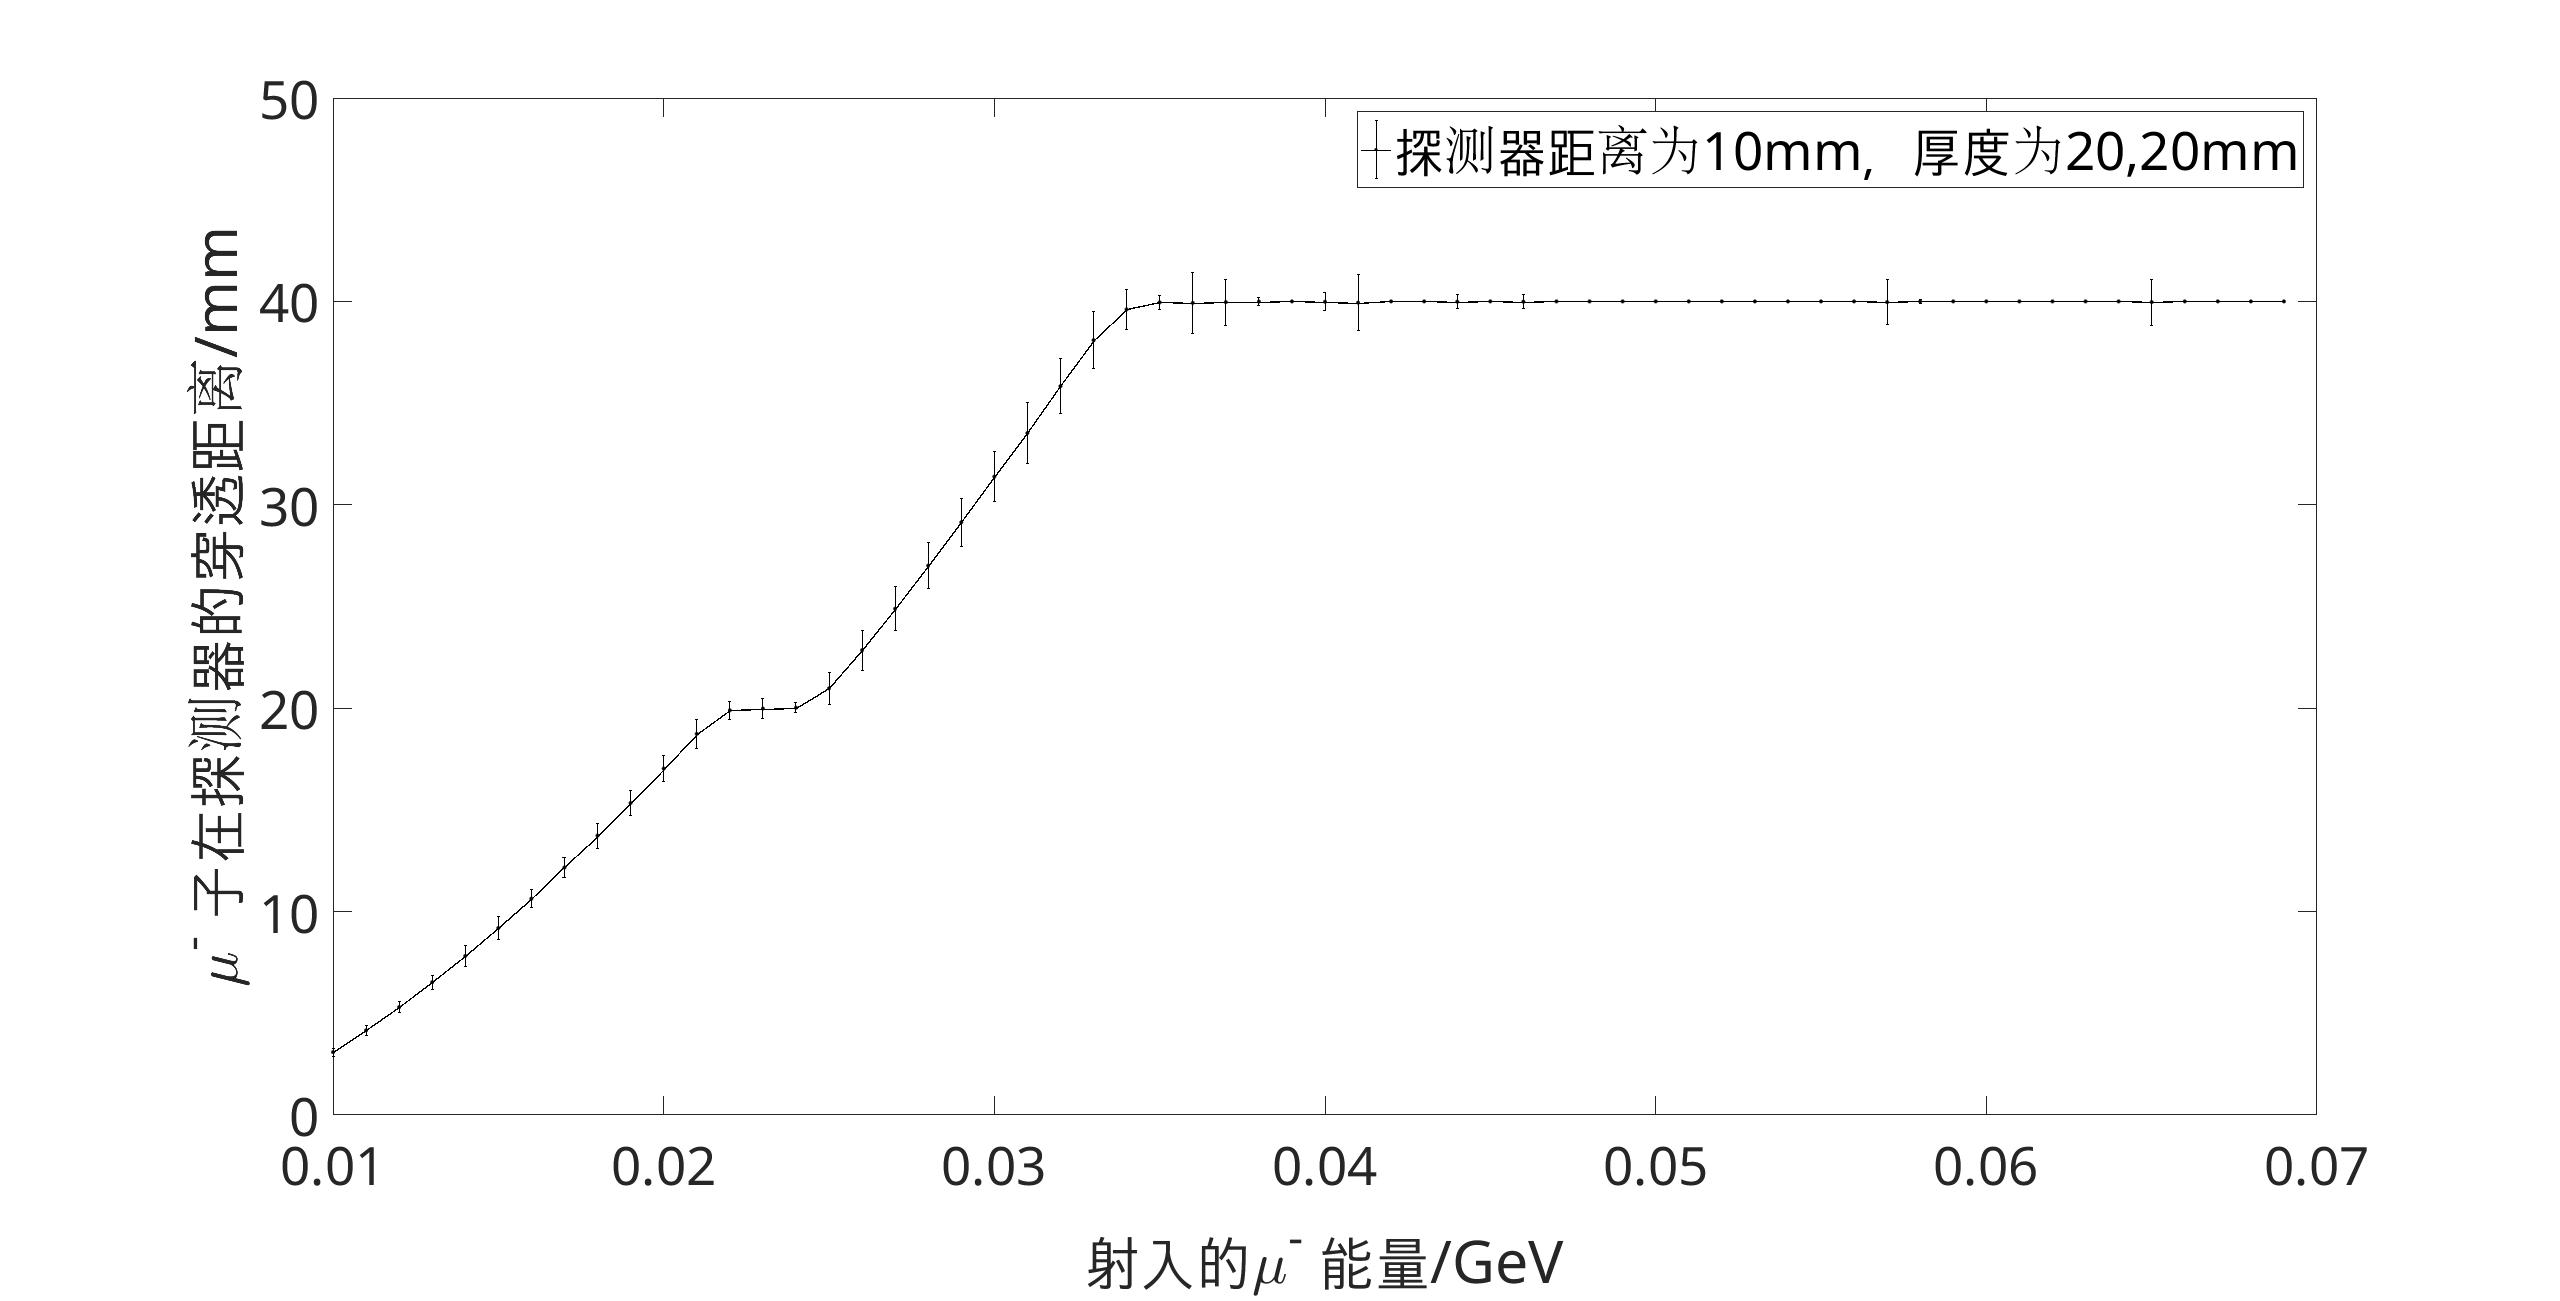
\includegraphics[width=100mm,height=50mm]{pic/de_distant_dis_10_se_20.jpg}
    \caption{缪子在探测器中穿透距离随着入射的缪子能量的变化曲线}\label{di1020}
\end{figure}


如图\ref{di1020}所示,该曲线有两个平台。第一个平台之前,上升曲线上的数据点所对应的穿透距离小于20$mm$,这是因为缪子能量较低时会在第一块探测器板中衰变。第一个平台上的数据点对应的缪子均在第一块探测器板与第二块探测器板间的空空隙中衰变。该图表示缪子在探测器中穿透距离随着入射的缪子能量的变化,由图可以看出第一个上升曲线的穿透距离小于20mm,说明缪子在第一个探测器中衰变,说明极低能的缪子会在第一个探测器中衰变,然后经过一个平台,到达第二个探测器中。之所以出现平台是因为我们只统计了缪子在探测器中运行距离,中间平台说明缪子需要耗费一定的能量才能到达第二个探测器中。
%需要说明的一点是为什么穿透距离到达了探测器的总厚度的时候,还会有方差不为0,这就表明了高能量的缪子在探测器衰变的几率已经很小了,已经跑出探测器了。但是高能量的缪子还是有可能在探测器中衰变,一旦衰变,穿透距离不等于探测器厚度,那么平均值也就比厚度小,这样绝大部分的穿透距离为厚度,这样方差就不为0了,由此造成的方差也可能会很大。\\


\begin{figure}[H]
    \centering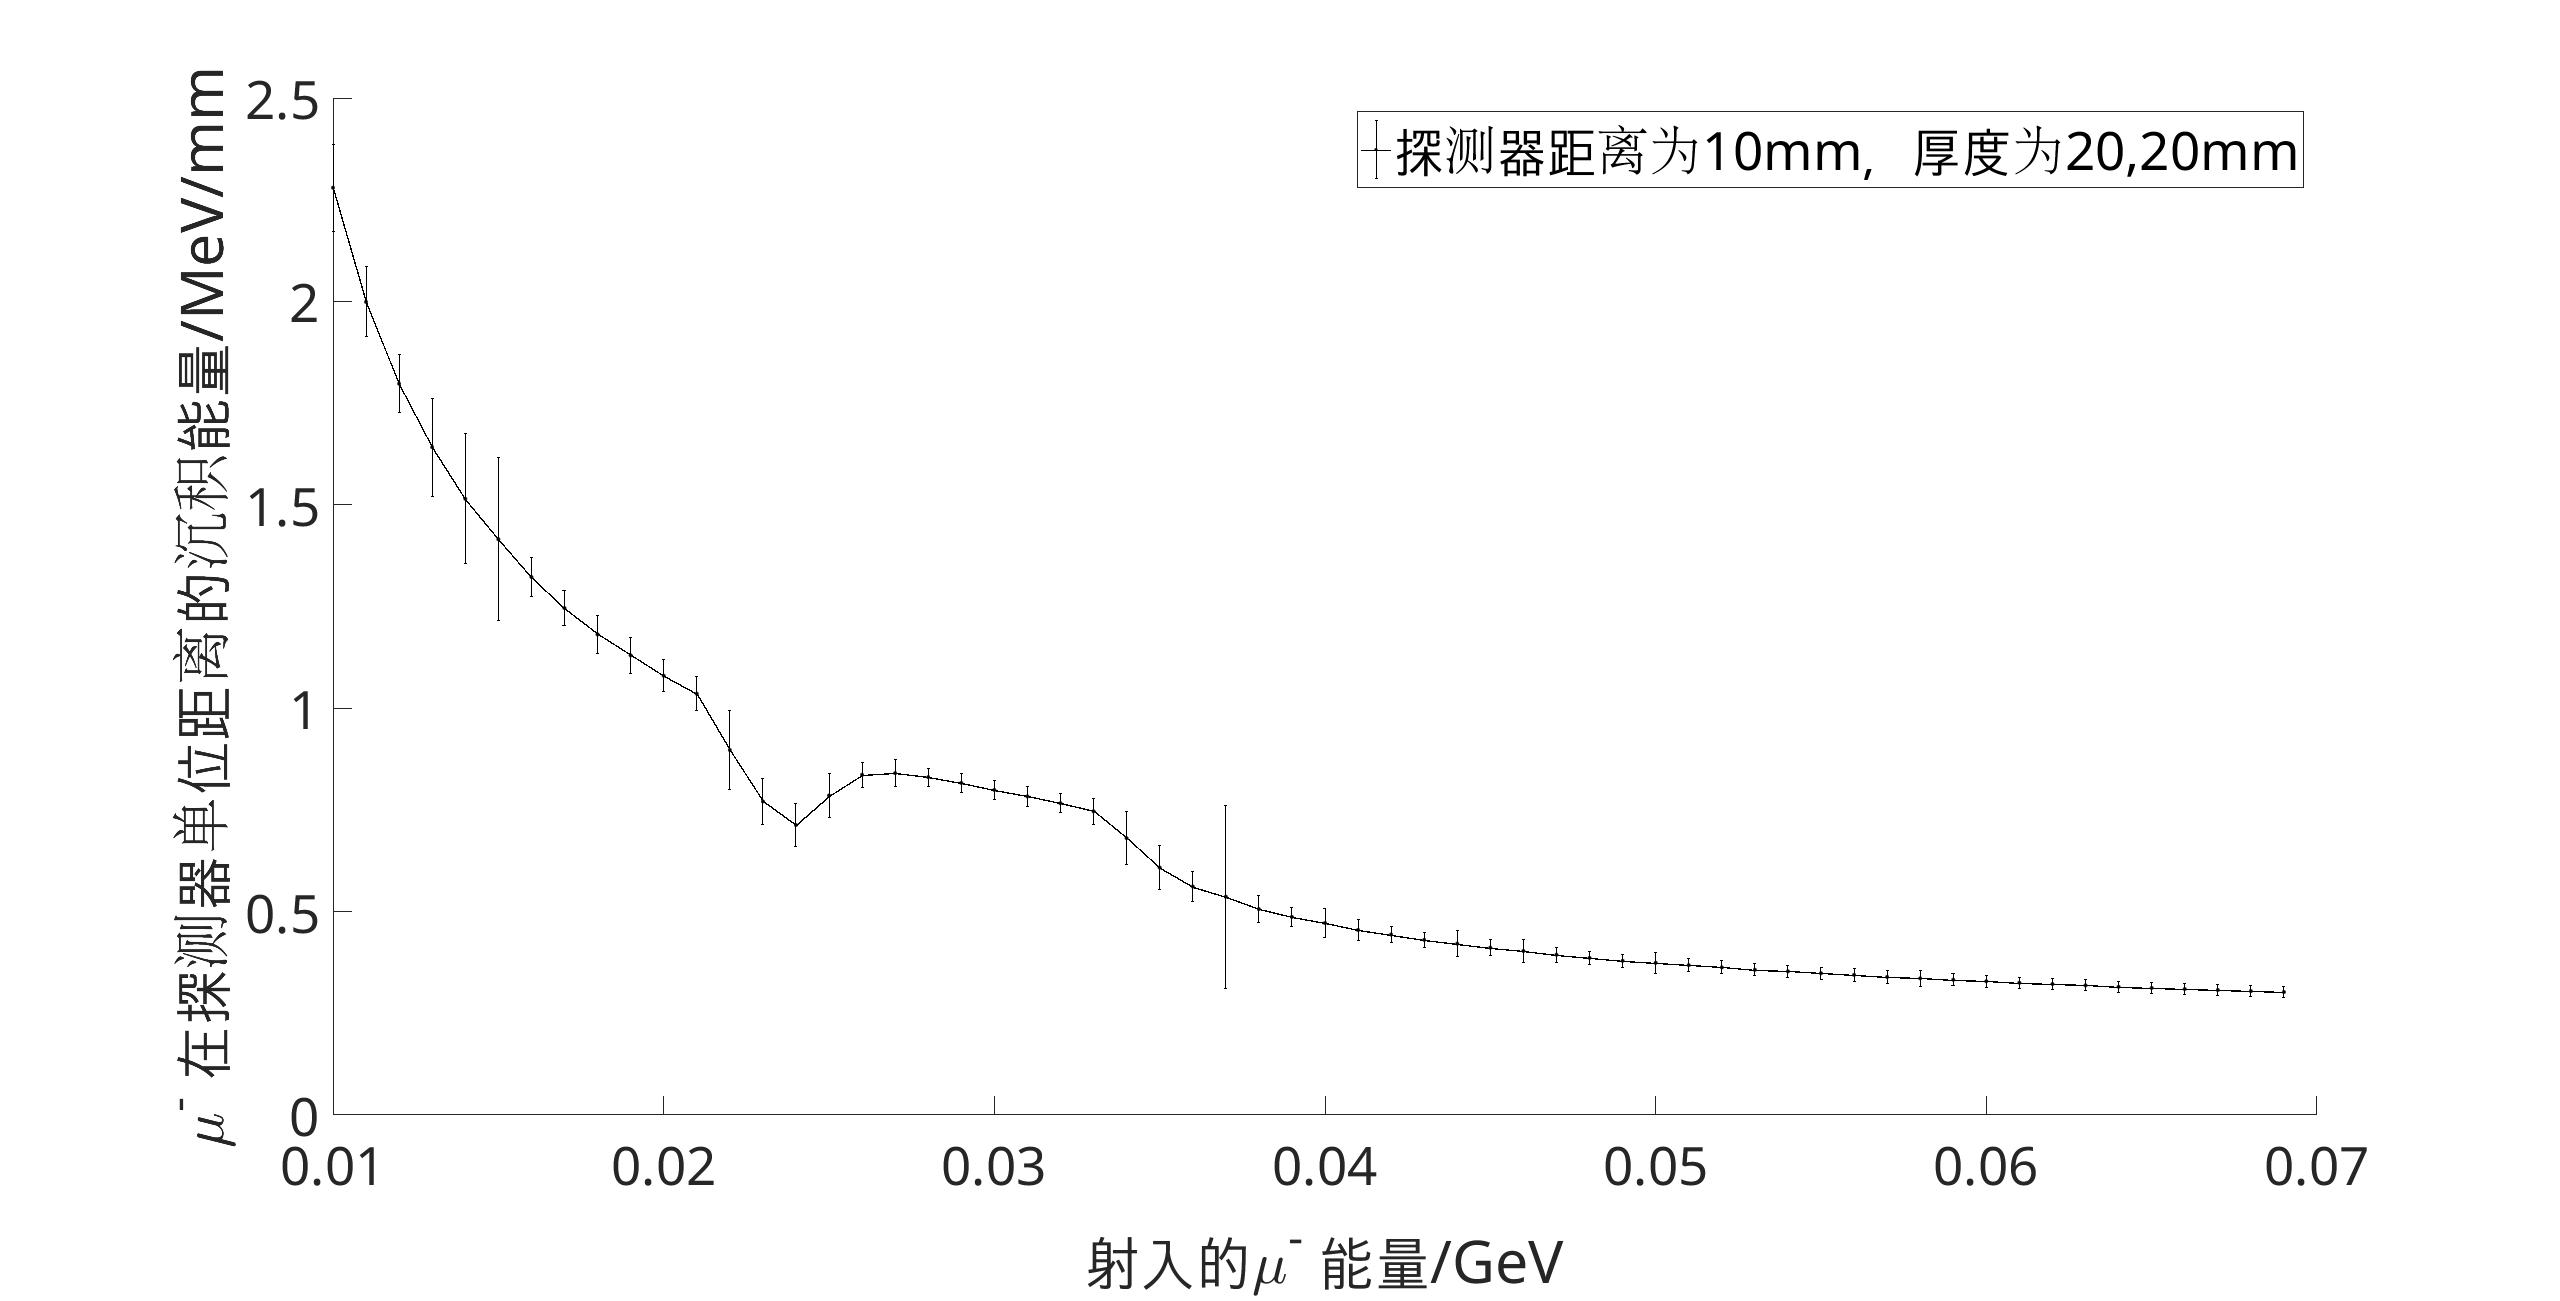
\includegraphics[width=0.6\textwidth]{pic/de_en_di_dis_10_se_20.jpg}
    \caption{缪子在探测器中单位距离沉积能量随着入射的缪子能量的变化曲线}\label{en_di1020}
\end{figure}


如图\ref{en_di1020}所示,缪子在探测器中单位距离沉积能量大体上随着入射缪子的能量递减,这是因为当能量的较小时,缪子在第一块探测器中衰变,释放能量可以通过$E=mc^2$直接由衰变前后的质量差算出,但是入射缪子的能量越大,在衰变前行进的距离越长,因此在释放能量一定的情况下单位距离的能量沉积越大。当入射缪子的能量足够大时,缪子在穿过两块板前不会衰变,此时的能量沉积主要来源于缪子使闪烁体中的分子电离时损失的能量,此部分能量基本不随入射缪子的能量变化,因此在入射缪子能量较大时,探测器中单位距离沉积能量基本不变。此外,当入射缪子能量介于0.02GeV和0.03GeV间以及0.03GeV和0.04GeV间时,单位距离沉积能量有一个快速下降的过程,这时缪子恰好可以穿过上探测器板和下探测器板。\\

\begin{figure}[H]
    \centering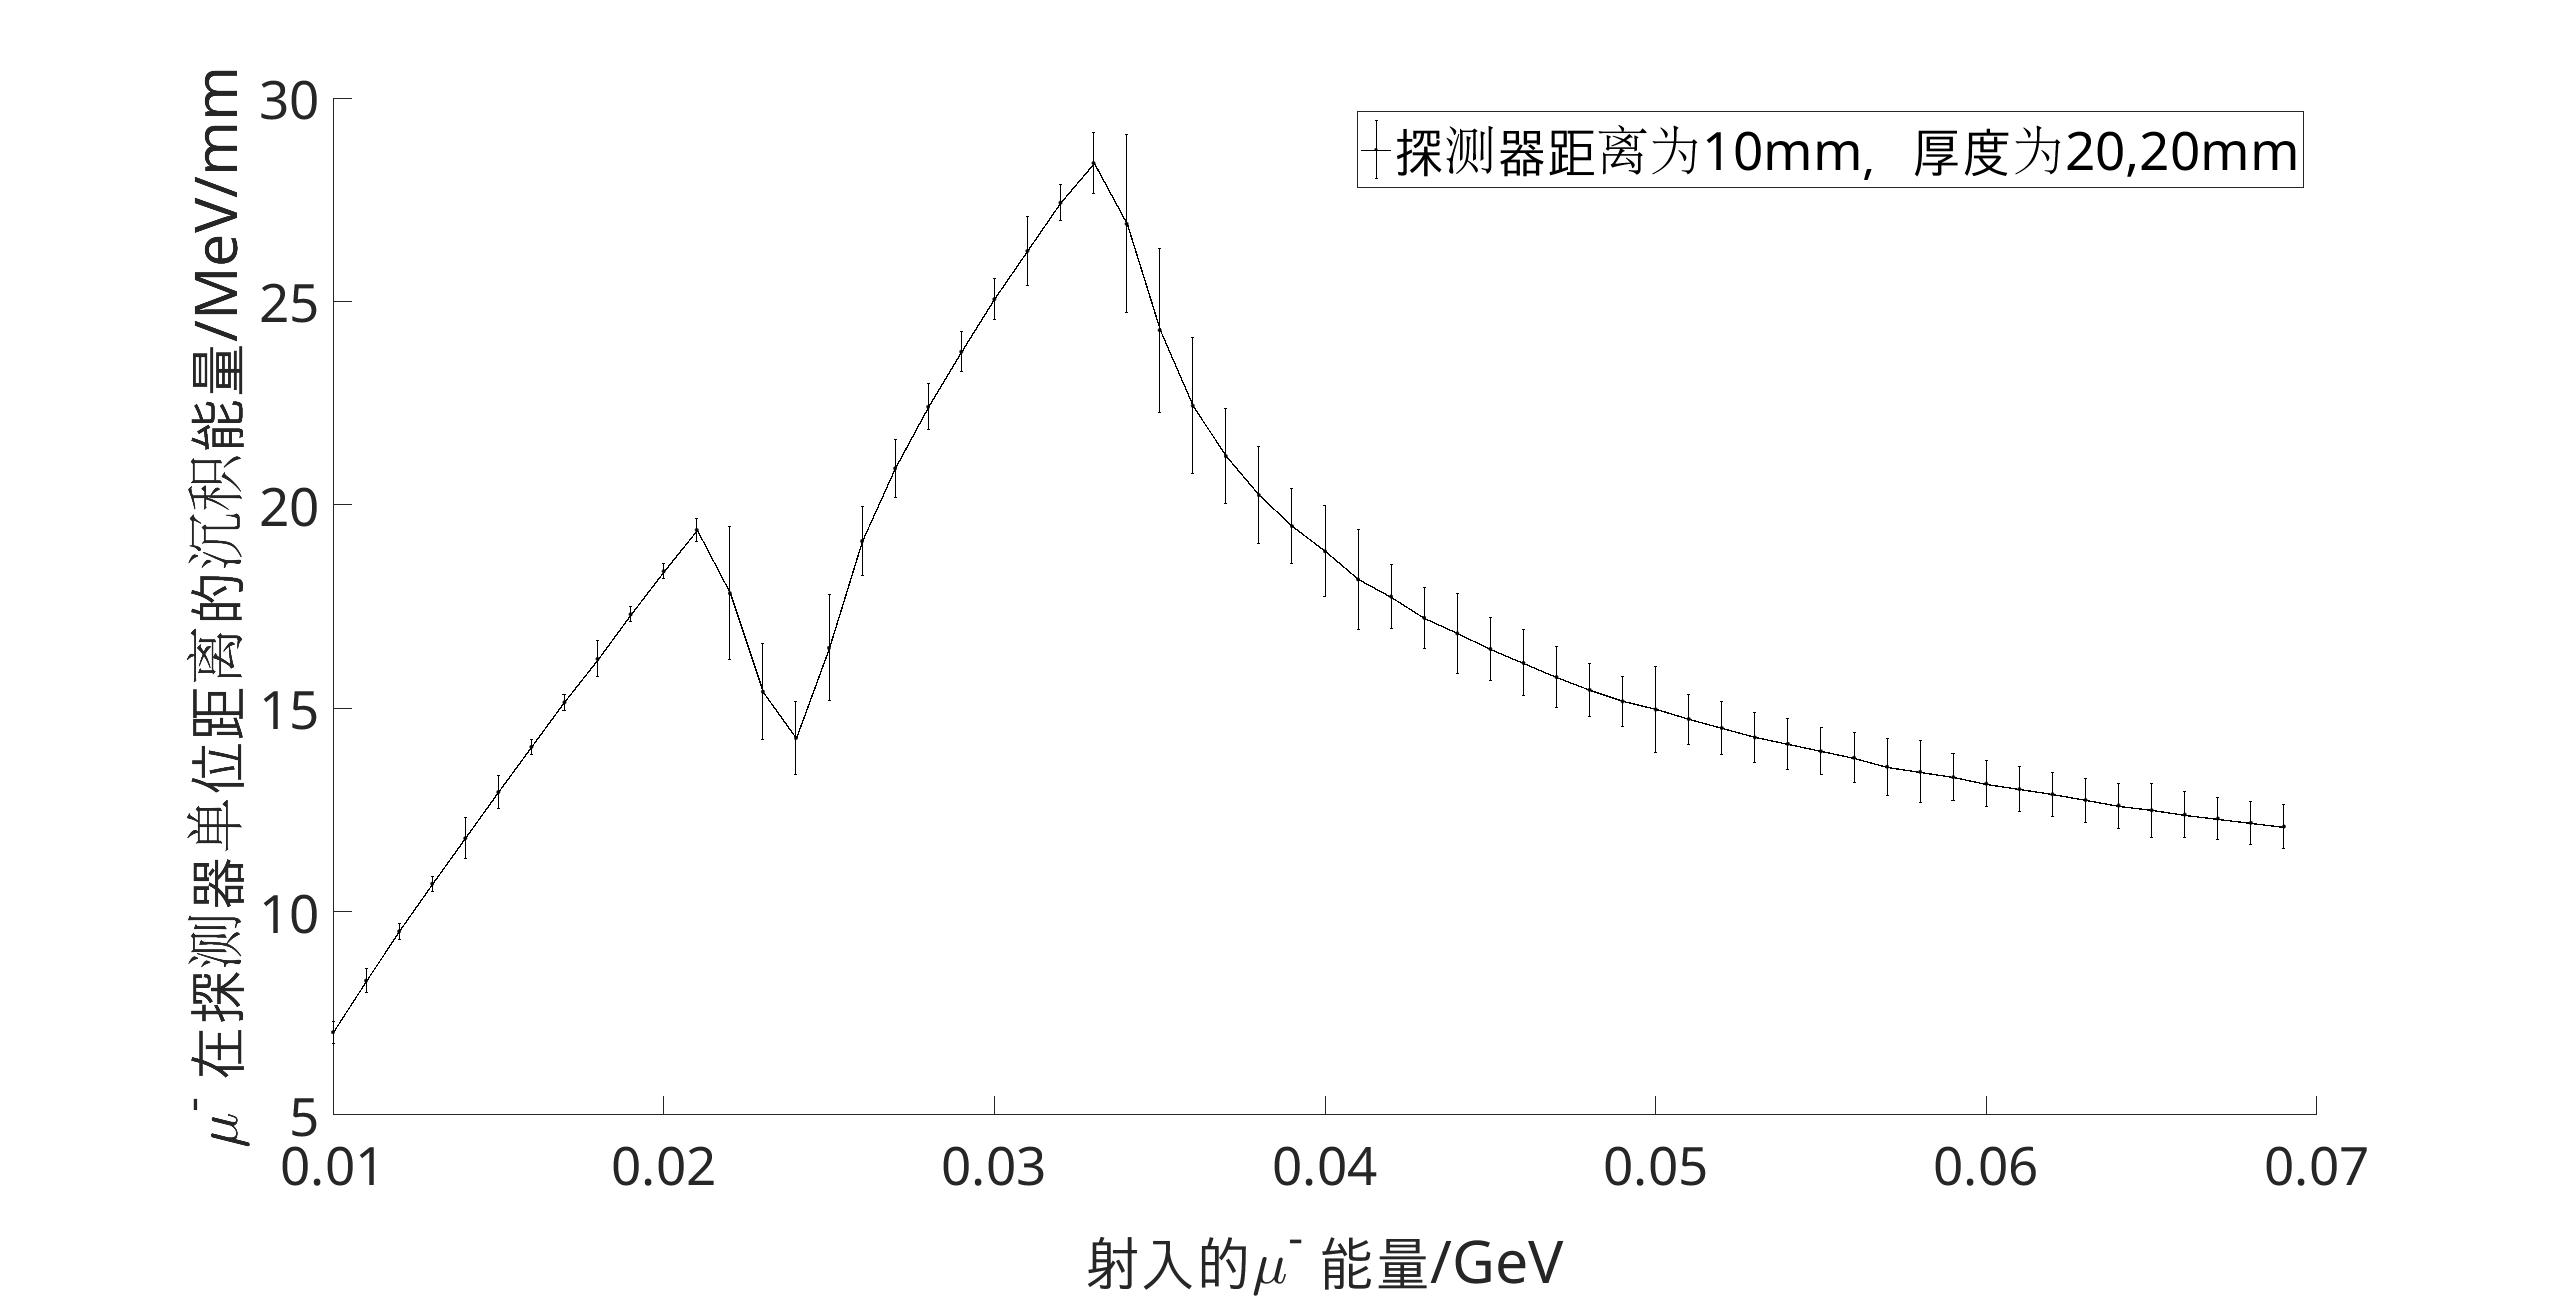
\includegraphics[width=0.6\textwidth]{pic/de_en_dis_10_se_20.jpg}
    \caption{缪子在探测器中沉积能量随着入射的缪子能量的变化曲线}\label{en1020}
\end{figure}

如图\ref{en1020}所示,缪子在探测器中沉积的能量随着入射缪子能量的变化总体上先增大再减小,并且有两处极大值。首先,在入射缪子的能量较小时,缪子在第一块探测器板中衰变,能量沉积即为衰变释放的能量与缪子初动能之和,因此入射缪子的能量越大,缪子初动能越大,能量沉积越大。当缪子的能量较大时,缪子不会在探测器板中衰变,此时能量沉积的主要来源是缪子动能在电离过程中的损失,此部分能量相较于衰变释放的能量要小得多,并且会随着缪子速度的增加而减小,因此入射缪子能量较大时,能量沉积下降。此外,曲线上的两个极大值分别对应着缪子在衰变前恰好穿过上探测器板时和恰好穿过下探测器板时的入射能量。由图可知,入射缪子的能量至少要达到0.02GeV才能通过上探测器板;入射缪子的能量至少要达到0.032GeV才能穿过下探测器板。当缪子在两块探测器板间的空隙中发生衰变时,衰变释放能并没有被包括在探测器能量沉积中,所以在0.02GeV和0.03GeV区间内有一段下降曲线。

\subsubsection{探测器厚度的影响}
接着我们调整了第二块探测器板的厚度并且绘制了不同厚度下入射缪子能量与缪子在探测器中的穿透距离的关系曲线。由图\ref{fig:di}可知,当入射缪子的能量很大时,缪子在探测器中的穿透距离不再改变,在曲线上对应一平台。这一平台的起点对应的缪子能量即为可以在探测器中衰变的缪子的最大入射能量。\ref{fig:di_linear}即为可以在探测器中发生衰变的缪子的最大入射能量与探测器下板厚度的关系曲线该曲线的\\


\begin{figure}[h]
\centering
    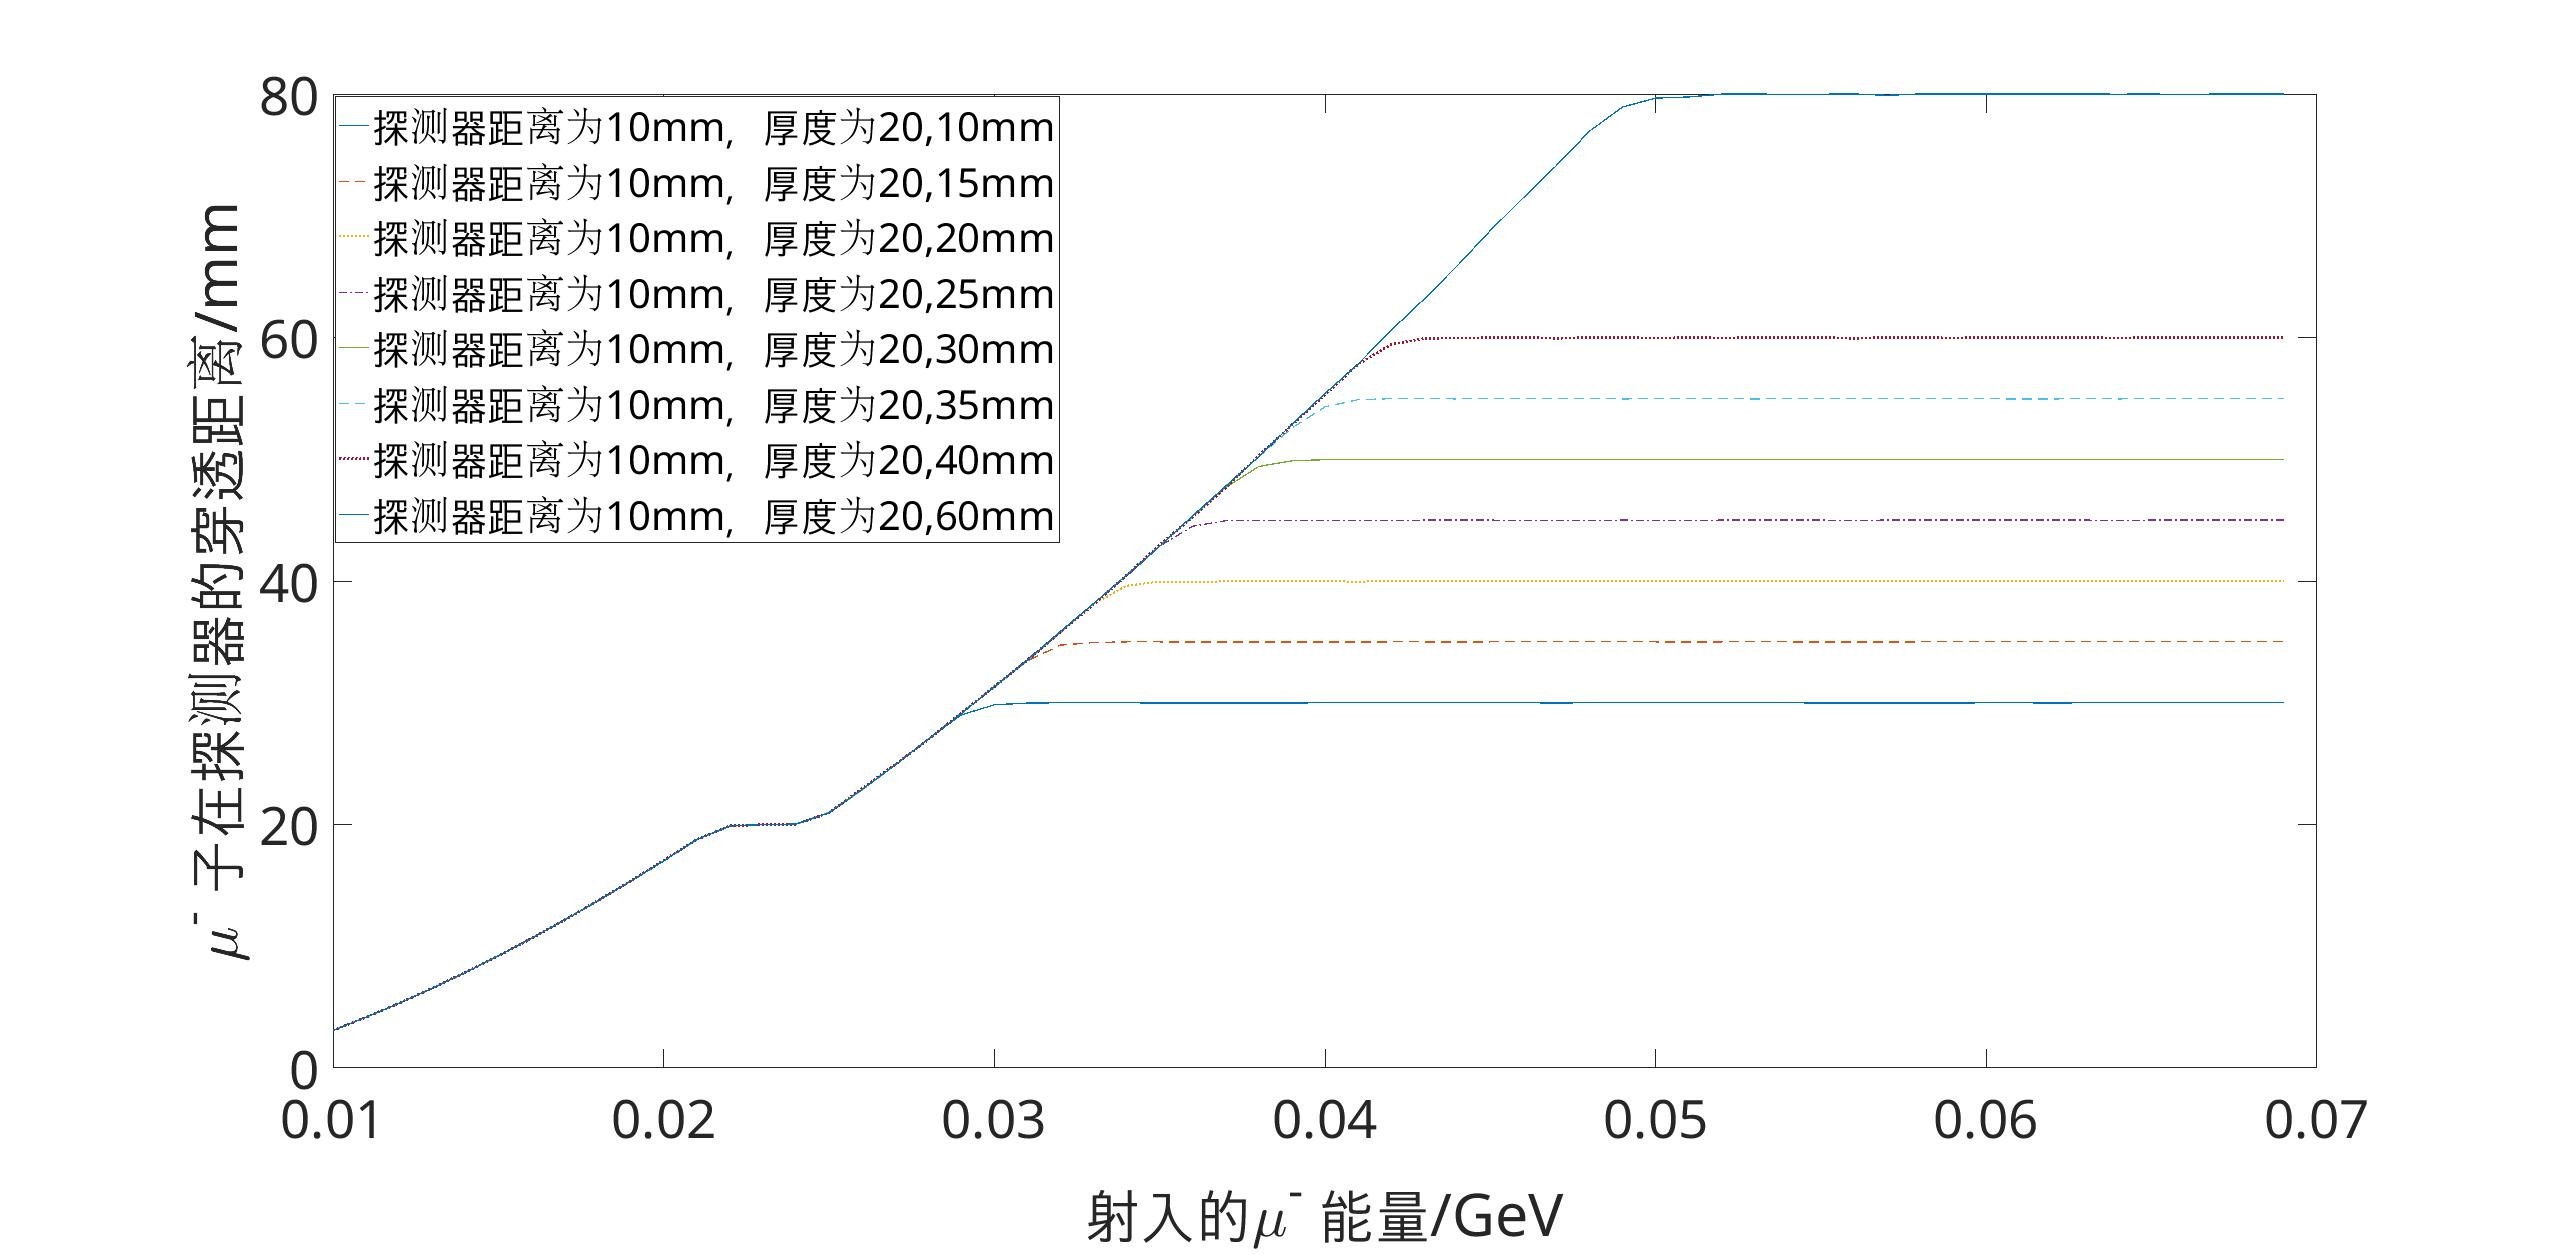
\includegraphics[width=0.6\textwidth]{pic/dis.jpg}
    \caption{厚度不同的穿透曲线}\label{fig:di}
    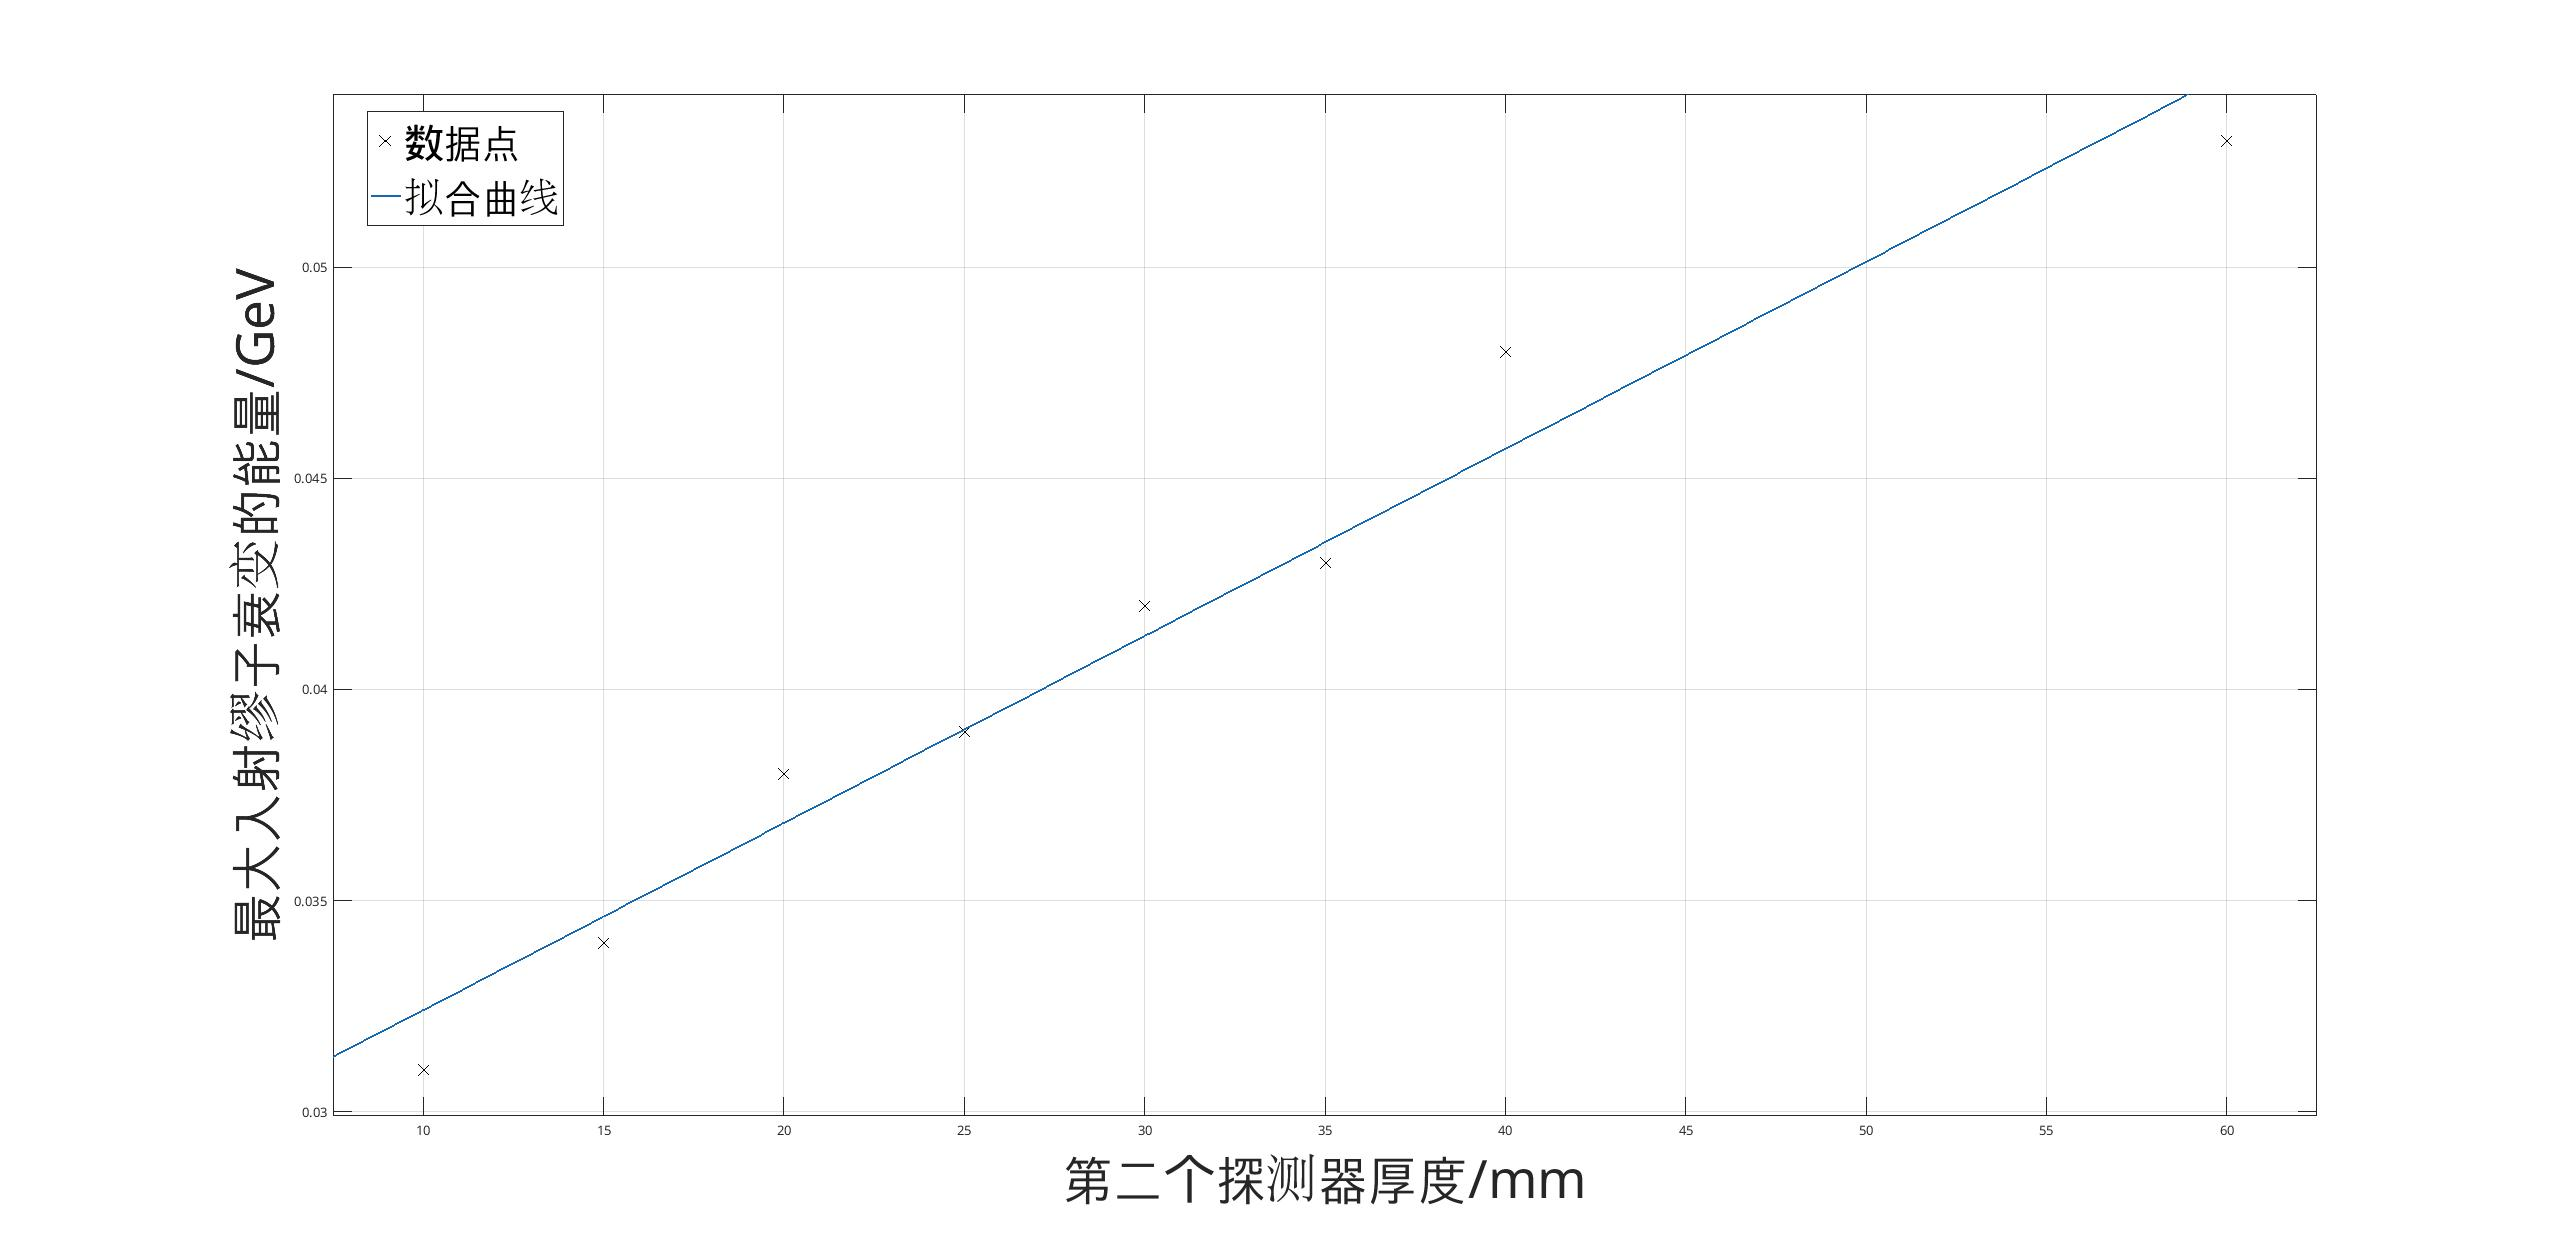
\includegraphics[width=0.6\textwidth]{pic/quxian.jpg}
    \caption{最大入射缪子衰变的能量和探测器厚度的关系}\label{fig:di_linear}
\end{figure}


拟合公式为 $k\times x + b$,其中$k = 0.000443,\ b= 0.02799$,R-square:0.9961\\


由这些参数可以知道在第二个探测器最大入射缪子衰变的能量和探测器厚度基本是线性关系,所以我们可以调控第一个探测器的厚度来控制缪子在第二个探测器衰变的最小能量,通过调控第二个探测器的厚度来控制缪子在第二个探测器衰变的最大能量,考虑探测器的造价,我们可以让该能量区间对应缪子达到地球表面能量几率最大并且最经济的区间。\\

\begin{figure}[H]
\centering
    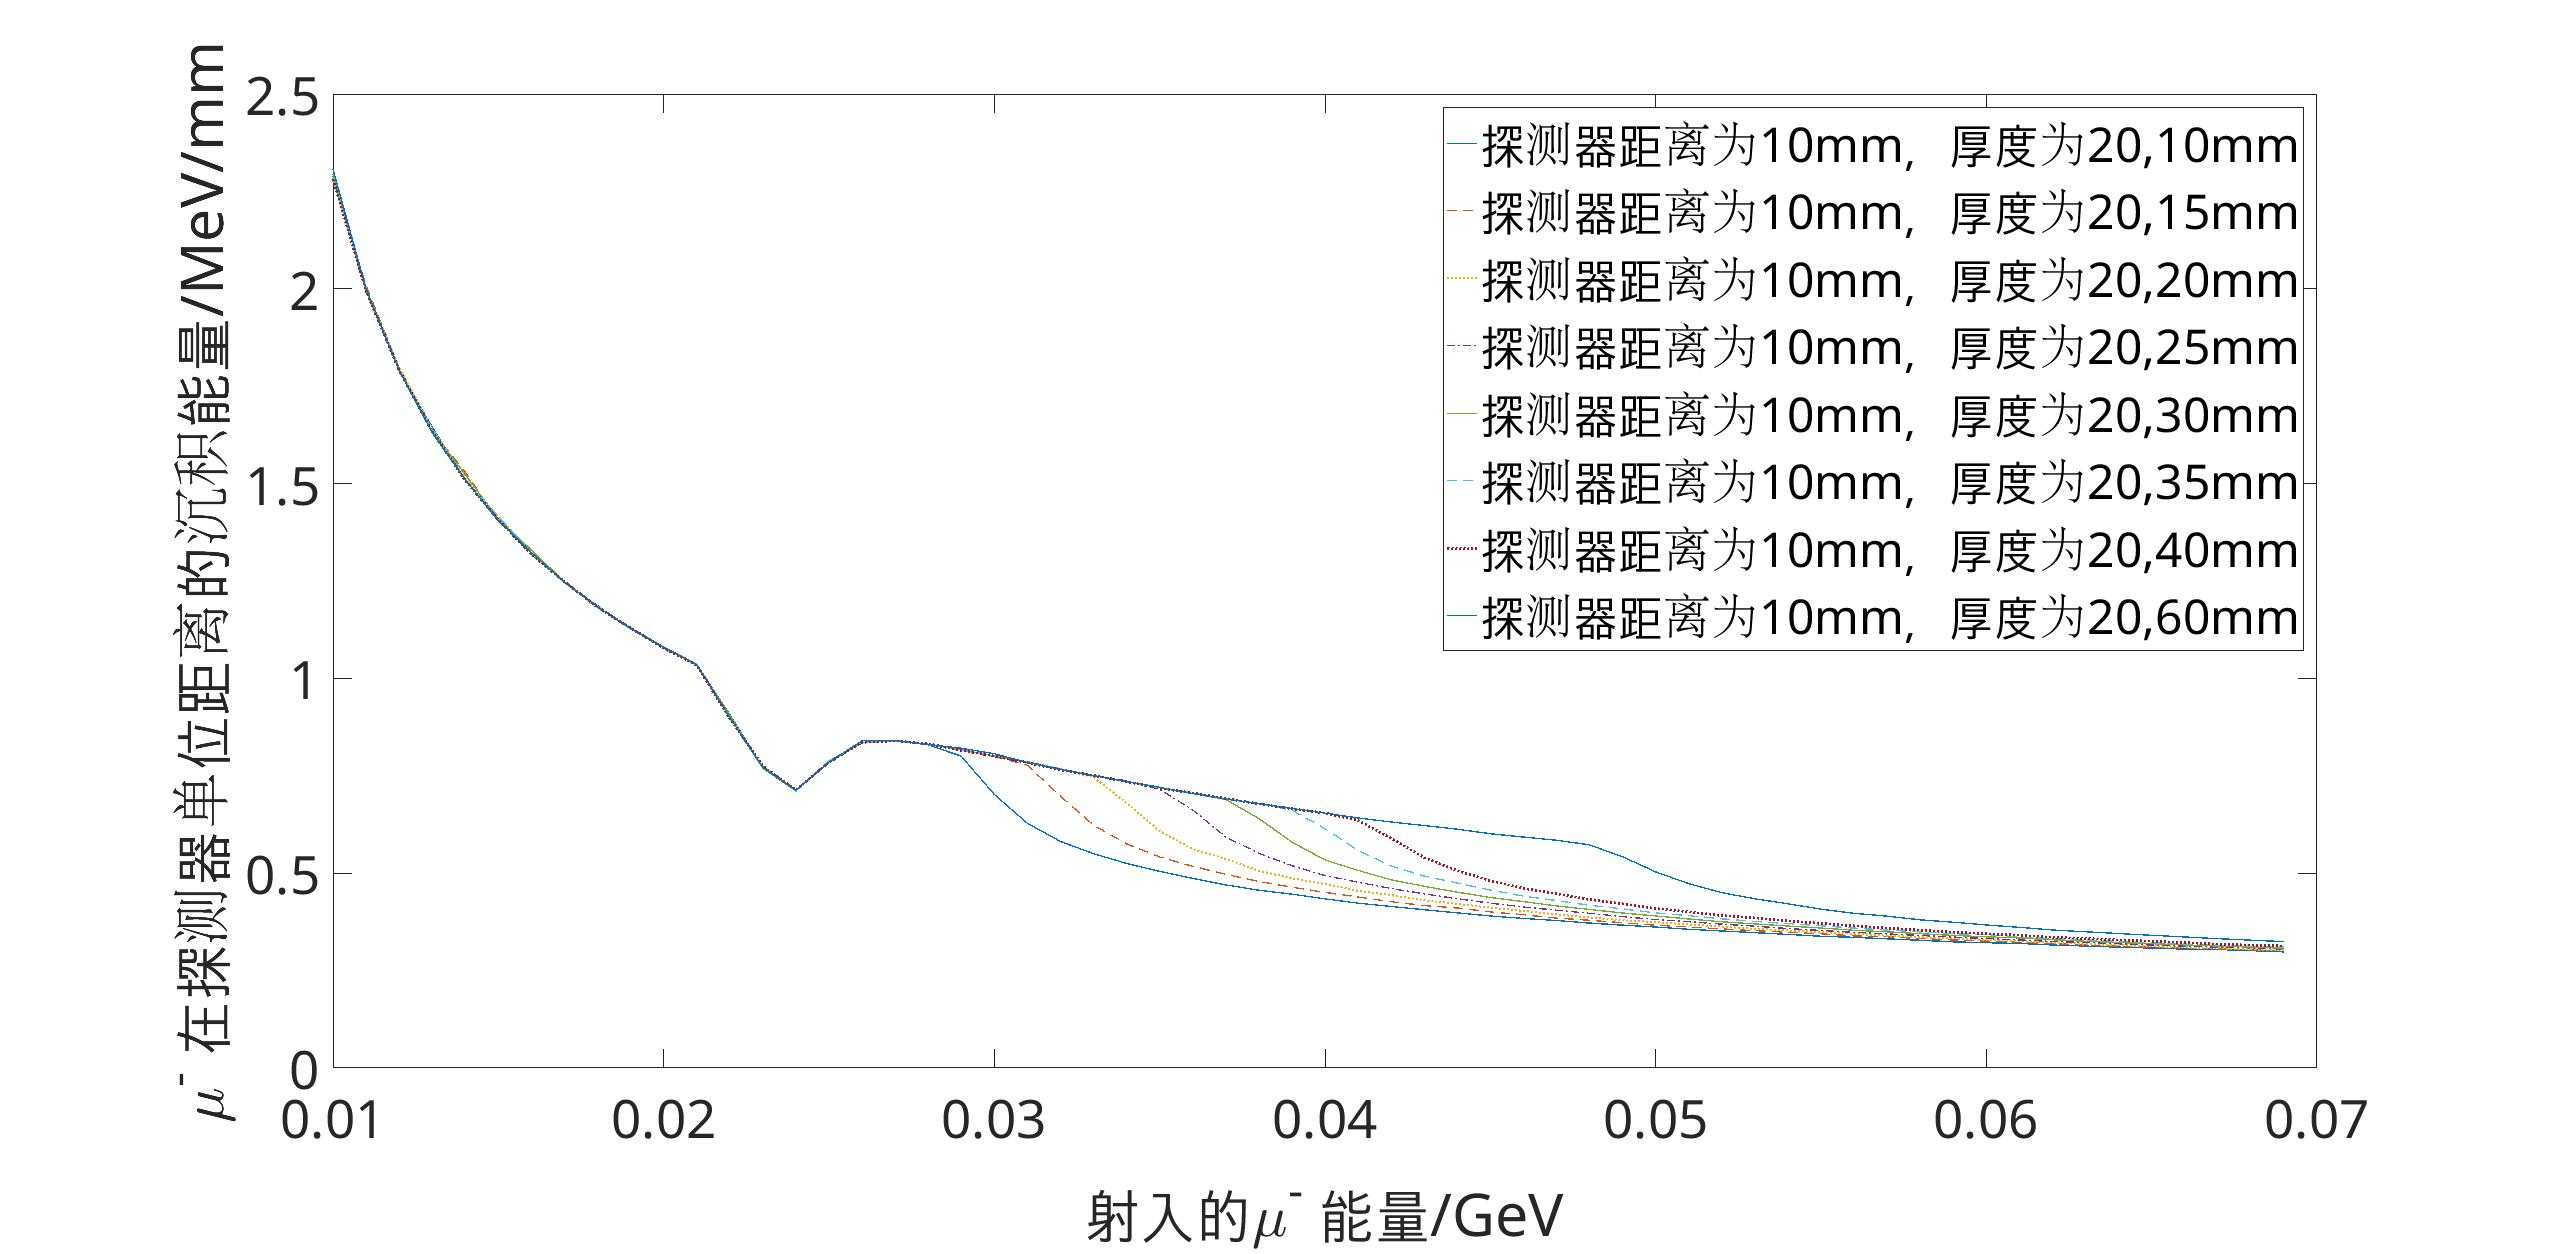
\includegraphics[width=0.6\textwidth]{pic/en_dis.jpg}
    \caption{厚度不同单位距离沉积能量的曲线}
\end{figure}

图曲线为缪子在探测器中单位距离沉积的能量与入射缪子能量的关系。




\subsection{缪子衰变统计}

如图所示,该曲线的横坐标是从缪子到达探测器到缪子衰变产生的光子射出探测器的时间差,纵坐标代表事例数。\\

\begin{figure}[H]
\centering
    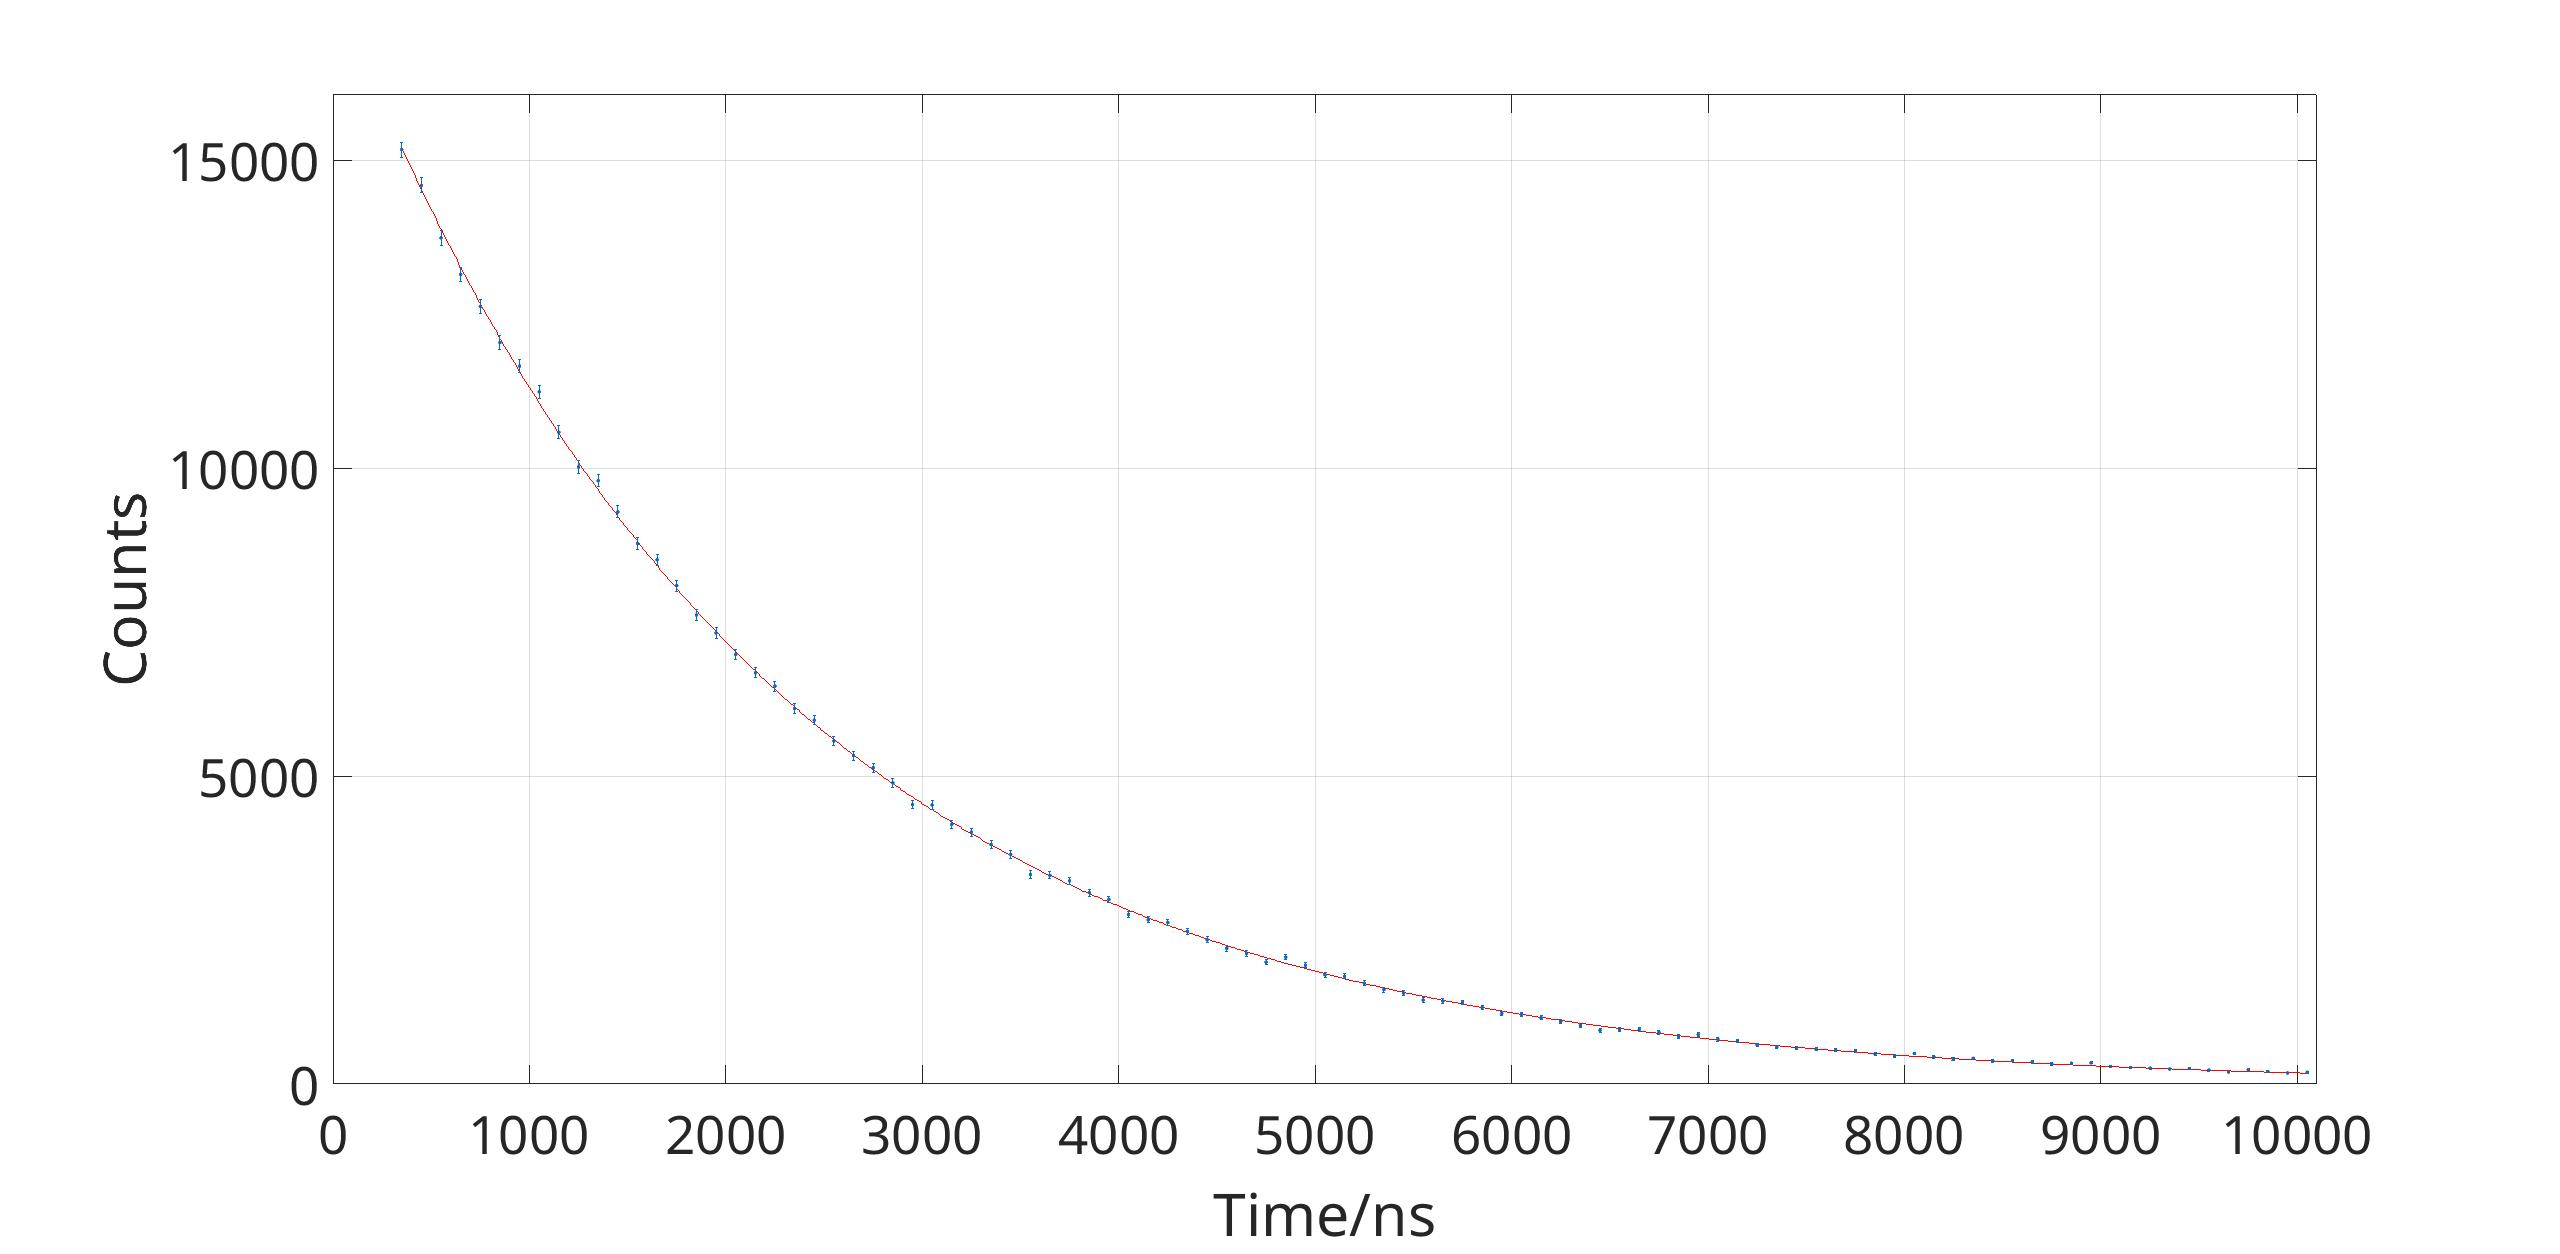
\includegraphics[width=0.6\textwidth]{pic/counts.jpg}
    \caption{缪子衰变时间统计图}
\end{figure}

拟合曲线$ a\times exp(-1/b\times x)+c$的参数(括号内是在95\%置性度水平拟合参数的浮动范围):
\begin{align}
      a & = & 1.783\times 10^4 & ~(1.777\times 10^4, 1.789\times 10^4)\\
       b & =  &    2203 & ~(2189, 2218)\\
       c & =  & -10.75 & ~(-33.95, 12.45)
\end{align}

sse: $2.5957\times 10^5$ rsquare: 0.9998  rmse: 52.2712\\
其中拟合参数b就是缪子的寿命,单位是ns。拟合可得精确值为2203 ns,与当前实验测量结果符合得非常好,误差控制在0.2937\%左右。

\section{结论}
我们用Geant4软件包实现了对缪子探测器探测结果的模拟,并初步讨论了模拟结果的物理含义,获得了缪子寿命测量的谱形。该模拟过程不仅可以对探测器的实际搭建起到指导作用,并为实际探测中的数据提供比对样本,更能够深入学生对探测器物理过程的理解,具有深远的教学意义。

\section{致谢}
该成果受到中山大学本科生科研项目的支持,同时受到中山大学“百人计划二期”高层次人才计划支持。感谢2016年基本粒子与相互作用协同创新中心年会暨``牡丹江合作组学术会议''上各兄弟高校支持中山大学高能物理学科建设,尤其感谢武汉大学周详博士和张振宇博士对该工作给予的帮助和鼓励。

%\newpage
\begin{thebibliography}{123456}
\bibitem {3}https://en.wikipedia.org/wiki/Muon

%\cite{Agostinelli:2002hh}
\bibitem{Agostinelli:2002hh}
  S.~Agostinelli {\it et al.} [GEANT4 Collaboration],
  %``GEANT4: A Simulation toolkit,''
  Nucl.\ Instrum.\ Meth.\ A {\bf 506}, 250 (2003).
  doi:10.1016/S0168-9002(03)01368-8
  %%CITATION = doi:10.1016/S0168-9002(03)01368-8;%%
  %8649 citations counted in INSPIRE as of 19 Jan 2018

%\cite{Aad:2010ah}
\bibitem{Aad:2010ah}
  G.~Aad {\it et al.} [ATLAS Collaboration],
  %``The ATLAS Simulation Infrastructure,''
  Eur.\ Phys.\ J.\ C {\bf 70}, 823 (2010)
  doi:10.1140/epjc/s10052-010-1429-9
  [arXiv:1005.4568 [physics.ins-det]].
  %%CITATION = doi:10.1140/epjc/s10052-010-1429-9;%%
  %1728 citations counted in INSPIRE as of 19 Jan 2018

%\cite{Abdullin:2011zz}
\bibitem{Abdullin:2011zz}
  S.~Abdullin {\it et al.} [CMS Collaboration],
  %``The fast simulation of the CMS detector at LHC,''
  J.\ Phys.\ Conf.\ Ser.\  {\bf 331}, 032049 (2011).
  doi:10.1088/1742-6596/331/3/032049
  %%CITATION = doi:10.1088/1742-6596/331/3/032049;%%
  %140 citations counted in INSPIRE as of 19 Jan 2018

%\cite{Hrivnacova:2011zz}
\bibitem{Hrivnacova:2011zz}
  I.~Hrivnacova {\it et al.} [ALICE Collaboration],
  %``The ALICE Geant4 simulation,''
  J.\ Phys.\ Conf.\ Ser.\  {\bf 331}, 032016 (2011).
  doi:10.1088/1742-6596/331/3/032016
  %%CITATION = doi:10.1088/1742-6596/331/3/032016;%%
  %3 citations counted in INSPIRE as of 19 Jan 2018

%\cite{Clemencic:2011zza}
\bibitem{Clemencic:2011zza}
  M.~Clemencic {\it et al.} [LHCb Collaboration],
  %``The LHCb simulation application, Gauss: Design, evolution and experience,''
  J.\ Phys.\ Conf.\ Ser.\  {\bf 331}, 032023 (2011).
  doi:10.1088/1742-6596/331/3/032023
  %%CITATION = doi:10.1088/1742-6596/331/3/032023;%%
  %411 citations counted in INSPIRE as of 19 Jan 2018

%\cite{Abe:2011ks}
\bibitem{Abe:2011ks}
  K.~Abe {\it et al.} [T2K Collaboration],
  %``The T2K Experiment,''
  Nucl.\ Instrum.\ Meth.\ A {\bf 659}, 106 (2011)
  doi:10.1016/j.nima.2011.06.067
  [arXiv:1106.1238 [physics.ins-det]].
  %%CITATION = doi:10.1016/j.nima.2011.06.067;%%
  %511 citations counted in INSPIRE as of 19 Jan 2018

%\cite{Ayres:2004js}
\bibitem{Ayres:2004js}
  D.~S.~Ayres {\it et al.} [NOvA Collaboration],
  %``NOvA: Proposal to Build a 30 Kiloton Off-Axis Detector to Study $\nu_{\mu} \to \nu_e$ Oscillations in the NuMI Beamline,''
  hep-ex/0503053.
  %%CITATION = HEP-EX/0503053;%%
  %665 citations counted in INSPIRE as of 19 Jan 2018

\bibitem {8} Agostinelli S, Allison J, Amako K a, et al. Geant4—a simulation toolkit. Nuclear instruments and methods in physics research section A: Accelerators, Spectrometers, Detectors and Associated Equipment, 2003, 506(3):250–303.

\bibitem {4}J. Beringer et al. (Particle Data Group), PR D86, 010001 (2012) (URL: http://pdg.lbl.gov)
\bibitem {6}Metropolis N, Ulam S. The monte carlo method[J]. Journal of the American statistical association, 1949, 44(247): 335-341.

\bibitem {2}林延畅, 陈少敏, 高原宁,等. μ子寿命测量与高能物理实验创造性人才的培养[J]. 实验技术与管理, 2008, 25(9):34-37.
\bibitem {7}苏恒. 基于Geant4的ARGO实验探测器模拟程序[D]. 山东大学, 2009.
\bibitem {5}吴雨生, 吕治严, 李数,等. 一种简便的$\mu$子寿命测量实验设计[J]. 中国科学技术大学学报, 2010, 40(6):608-611.
\bibitem {1}谢红刚, 牛胜利, 黄流兴. Geant4模拟半导体器件的单粒子效应[J]. 清华大学学报(自然科学版), 2007, 47(s1):1035-1039.

\end{thebibliography}


\newpage

我们以$\mu^-$粒子为例,模拟输出单个事例历经的物理过程如下:\\
G4Track Information: Particle = mu-, Track ID = 1,  Parent ID = 0\\
\begin{center}
\begin{tabular}{|c|c|c|c|c|c|}
 X(mm) & Y(mm) & Z(mm) & KinE(MeV)  & NextVolume & ProcName\\
 0    &  0      &  100  &  10   &       World &  initStep\\
 0.26 & -0.252  &  30.4 & 9.92  &        World &  muIoni\\
0.277  & -0.289 &   26 &  9.92  &   Al2O32 & Transportation\\
0.279 & -0.295  &  25.4 & 8.39  &     Al2O32  & muIoni\\
0.33 & -0.314  &    25 &  7.02 &    muondector2  & Transportation\\
0.714 &  -0.55 &  21.8 &  0    &    muondector2  & muIoni\\
0.714 & -0.55  &   21.8 &  0     & muondector2 & Scintillation

\end{tabular}
\end{center}

%anti\_nu\_e nu\_mu经历Transportation\\

G4Track Information:   Particle = nu\_mu,   Track ID = 21,   Parent ID = 1\\

\begin{center}
\begin{tabular}{|c|c|c|c|c|c|}
X(mm) & Y(mm) & Z(mm) & KinE(MeV)  & NextVolume & ProcName\\
0.714 & -0.55 &  21.8 & 30.7 &   muondector2 & initStep\\
-19.9 &   -51.2  &    100   &   30.7  & OutOfWorld  & Transportation

\end{tabular}
\end{center}

G4Track Information:   Particle =  anti\_nu\_e,   Track ID = 20,   Parent ID = 1\\

\begin{center}
\begin{tabular}{|c|c|c|c|c|c|}
X(mm) & Y(mm) & Z(mm) & KinE(MeV)  & NextVolume & ProcName\\
0.714 & -0.55 &  21.8 & 24.4 &   muondector2 & initStep\\
-24.6 &   45.6  &    100   &   24.4  & OutOfWorld  & Transportation

\end{tabular}
\end{center}

%电子在塑料闪烁体中经历 eBrem 和 Cerenkov 释放大量光子,同时经过 eIoni 释放低能电子和 gamma 光子,最后经历Scintillation\\

%电子在空气中也是经历eIoni 和Scintillation 闪烁过程 eIonic 过程会放出低能电子。\\

G4Track Information:   Particle = e-,   Track ID = 19,   Parent ID = 1\\

\begin{center}
\begin{tabular}{|c|c|c|c|c|c|}

X(mm)  &  Y(mm)  &  Z(mm) & KinE(MeV)  &  NextVolume & ProcName\\
0.714  &  -0.55   &  21.8 &    50  &    muondector2 & initStep\\
1.44  &  -0.158    &   19     &  47.7   & muondector2 & eBrem\\
3.74   &   1.76  &   8.21   &   45.5     &  muondector2 & Cerenkov\\
4.37    & 2.3 &  5  &  44.8   &     Al2O32  & Transportation\\
4.53  &   2.37  &  4 & 44.3  &     World & Transportation\\
5.77  &  3.07  & -4.88   &  38   &  Al2O31 & eBrem (已经到达了)\\
5.85  & 3.08 & -5.55  &   34.3   &  muondector1 & eIoni(已经到达了 0.0896MeV)\\
\end{tabular}
\end{center}


G4Track Information:   Particle = e-,   Track ID = 577,   Parent ID = 19\\

\begin{center}
\begin{tabular}{|c|c|c|c|c|c|}
X(mm)  &  Y(mm)  &  Z(mm) & KinE(MeV)  &  NextVolume & ProcName\\
5.85  & 3.08  &  -5.55    &  3.55    & muondector1  & initStep\\
11.7  &  -1.3 & -14.7    &   0.448    & muondector1 & eIoni\\
12 & -1.15 & -15.1   &    0   &  muondector1  & Cerenkov\\
 12  & -1.15  & -15.1    &   0     &  muondector1  & Scintillation

\end{tabular}
\end{center}

\end{CJK}
\end{document}

